% -------------------------------------------------------------------
% CV LaTeX — Préversion avant formation
% Auteur : Philippe Thomas Savard
% Licence : Apache 2.0
% -------------------------------------------------------------------

\documentclass[11pt,a4paper]{article}

% -------------------------------------------------------------------
% Packages essentiels
% -------------------------------------------------------------------
\usepackage[utf8]{inputenc}
\usepackage[T1]{fontenc}
\usepackage{geometry}
\usepackage{setspace}
\usepackage{titlesec}
\usepackage{graphicx}
\geometry{margin=1in}
\setstretch{1.15}

% -------------------------------------------------------------------
% hyperref DOIT être le dernier package chargé
% -------------------------------------------------------------------
\usepackage{hyperref}
\hypersetup{
    colorlinks=true,
    urlcolor=blue,
    linkcolor=blue,
    citecolor=blue
}

% -------------------------------------------------------------------
% Mise en forme des titres
% -------------------------------------------------------------------
\titleformat{\section}{\large\bfseries}{\thesection}{1em}{}
\titleformat{\subsection}{\normalsize\bfseries}{\thesubsection}{1em}{}

% -------------------------------------------------------------------
% Début du document
% -------------------------------------------------------------------
\begin{document}

% -------------------------------------------------------------------
% En-tête du CV
% -------------------------------------------------------------------
\begin{center}
    {\LARGE \textbf{Parcours professionnel (CV)}}\\[0.5cm]

    \textbf{Philippe Thomas Savard}\\
    4-5354 rue du Menuet, G6X 2Y6, Lévis, Québec\\
    \href{mailto:philippethomassavard@gmail.com}{philippethomassavard@gmail.com}\\[0.3cm]

    \textit{Document sous licence Apache 2.0}\\[0.5cm]
\end{center}

% -------------------------------------------------------------------
% Déclaration d'authenticité
% -------------------------------------------------------------------
\noindent
\textbf{Déclaration :}  
Le présent document constitue une préversion authentique de mon parcours professionnel, académique et autodidacte.  
Il reflète fidèlement mon expérience réelle, mes apprentissages personnels et mes réalisations techniques.  
Aucune information n’est figée : ce document est ouvert à la modification, à la mise à jour et à la contribution,  
conformément à la licence Apache 2.0.

Un dépôt GitHub associé contient l’ensemble des travaux, documents, scripts et validations mentionnés dans ce CV.  
Lien du dépôt : \url{https://github.com/2racinede4carreunivers-dev/porte_folio_savard.git}

\vspace{0.8cm}

% -------------------------------------------------------------------
% Introduction aux sections d'expérience
% -------------------------------------------------------------------
\noindent
Ce curriculum vitae présente mon parcours en deux volets complémentaires :

\begin{itemize}
    \item \textbf{Expérience professionnelle passée} : emplois, formations officielles, compétences techniques acquises en milieu de travail.
    \item \textbf{Expérience autodidacte et auto-pédagogique} : travaux personnels en mathématiques, géométrie, modélisation, DAO/CAO,  
    développement logiciel et formalisation scientifique.
\end{itemize}

\vspace{0.5cm}

% -------------------------------------------------------------------
% Section : Scolarité
% -------------------------------------------------------------------
\section*{Scolarité}

\begin{itemize}
    \item Diplôme d'études secondaires — Juin 2002
    \item Diplôme d'études professionnelles (DEP) — Électricité de chantier — 2006
    \item Études collégiales en génie civil — 4 sessions complétées sur 6
\end{itemize}

% -------------------------------------------------------------------
% Section : Expérience autodidacte et auto-pédagogique
% -------------------------------------------------------------------
\section*{Expérience autodidacte et auto-pédagogique}

\subsection*{Projet personnel en mathématiques et géométrie (2016 — aujourd'hui)}

Depuis mai 2016, je développe un projet scientifique complet portant sur :

\begin{itemize}
    \item l'hypothèse de Riemann,
    \item la mécanique harmonique du chaos discret,
    \item la géométrie du spectre des nombres premiers,
    \item une théorie unifiée reliant ces structures.
\end{itemize}

Travaux réalisés :

\begin{itemize}
    \item Conception de figures géométriques via \textbf{AutoCAD}, \textbf{Rhino/Grasshopper} et \textbf{TikZ}.
    \item Développement de scripts en \textbf{Python}, \textbf{LaTeX}, \textbf{HOL}, \textbf{Java}, \textbf{Markdown}, etc.
    \item Production de documents LaTeX explicatifs (PDF) sur la géométrie du spectre et la mécanique harmonique.
    \item Création d’outils web permettant à l’utilisateur d’interroger la théorie via trois IA spécialisées.
    \item Validation formelle par Isabelle/HOL :
    \begin{itemize}
        \item \texttt{methode\_spectral.thy}
        \item \texttt{methode\_de\_philippot.thy}
        \item \texttt{mecanique\_discret.thy}
    \end{itemize}
    \item Développement d’une axiomatisation géométrique inspirée de la méthode de pesée d’Archimède.
\end{itemize}

% Liens GitHub cliquables
\href{https://github.com/2racinede4carreunivers-dev/analyse-de-la-conjecture-zeta-riemann-savard.git}{Analyse Riemann} •
\href{https://github.com/2racinede4carreunivers-dev/porte_folio_savard.git}{Portfolio} •
\href{https://github.com/2racinede4carreunivers-dev/formation_evolutive_savard.git}{Formation}

% -------------------------------------------------------------------
% Section : Expérience professionnelle
% -------------------------------------------------------------------
\section*{Expérience professionnelle}

\subsection*{Assembleur — ABB (maintenant Hitachi) — Étés 2002, 2003, 2004}
\begin{itemize}
    \item Emploi étudiant à l'usine ABB (Hitachi) dans la région de Québec.
    \item Assemblage aux tables de production.
    \item Travail en milieu manufacturier industriel.
\end{itemize}

\subsection*{Électricien de chantier — Projets Le Symbiose et Le Sommet — Montréal}
\begin{itemize}
    \item Installation électrique sur chantiers résidentiels et commerciaux.
    \item Lecture de plans, câblage, raccordements et conformité aux normes.
\end{itemize}

\subsection*{Électricien — Marcel Pager Électricien — Province de Québec}
\begin{itemize}
    \item Installation de thermostats dans le cadre du programme Hydro-Québec Éconologie.
    \item Travail mobile à travers plusieurs régions du Québec.
\end{itemize}

\subsection*{Électricien de chantier — Luard Électrique — Lévis}
\begin{itemize}
    \item Participation au projet Le Sélection Lévis.
    \item Installation électrique complète sur chantier.
\end{itemize}

\subsection*{Installateur de piscines — Piscines Sansouci — Saint-Rédempteur (Lévis)}
\begin{itemize}
    \item Installation de piscines hors-terre et creusées.
    \item Service dans la région de Québec et Lévis.
\end{itemize}

\subsection*{Installateur de piscines — Piscine Concept Design Val-Bellaire — Poste actuel}
\begin{itemize}
    \item Installation de piscines hors-terre.
    \item Travail saisonnier spécialisé dans la région de Québec.
\end{itemize}

% -------------------------------------------------------------------
% Conclusion
% -------------------------------------------------------------------
\section*{Conclusion}

La présente version de mon curriculum vitæ constitue une préversion évolutive. 
Elle est conçue pour permettre au recruteur d’observer, au fil du temps, l’évolution de mon organisation personnelle, 
la progression de ma formation pédagogique qui débute au CFP Neufchâtel, ainsi que le parallèle entre mes apprentissages, 
mes projets autodidactes et mon parcours professionnel. 
Ce document continuera d’être mis à jour tout au long de ma formation et de mes réalisations techniques.

\vspace{0.8cm}

\noindent
\textbf{Signature :}

\vspace{0.4cm}

\begin{center}
    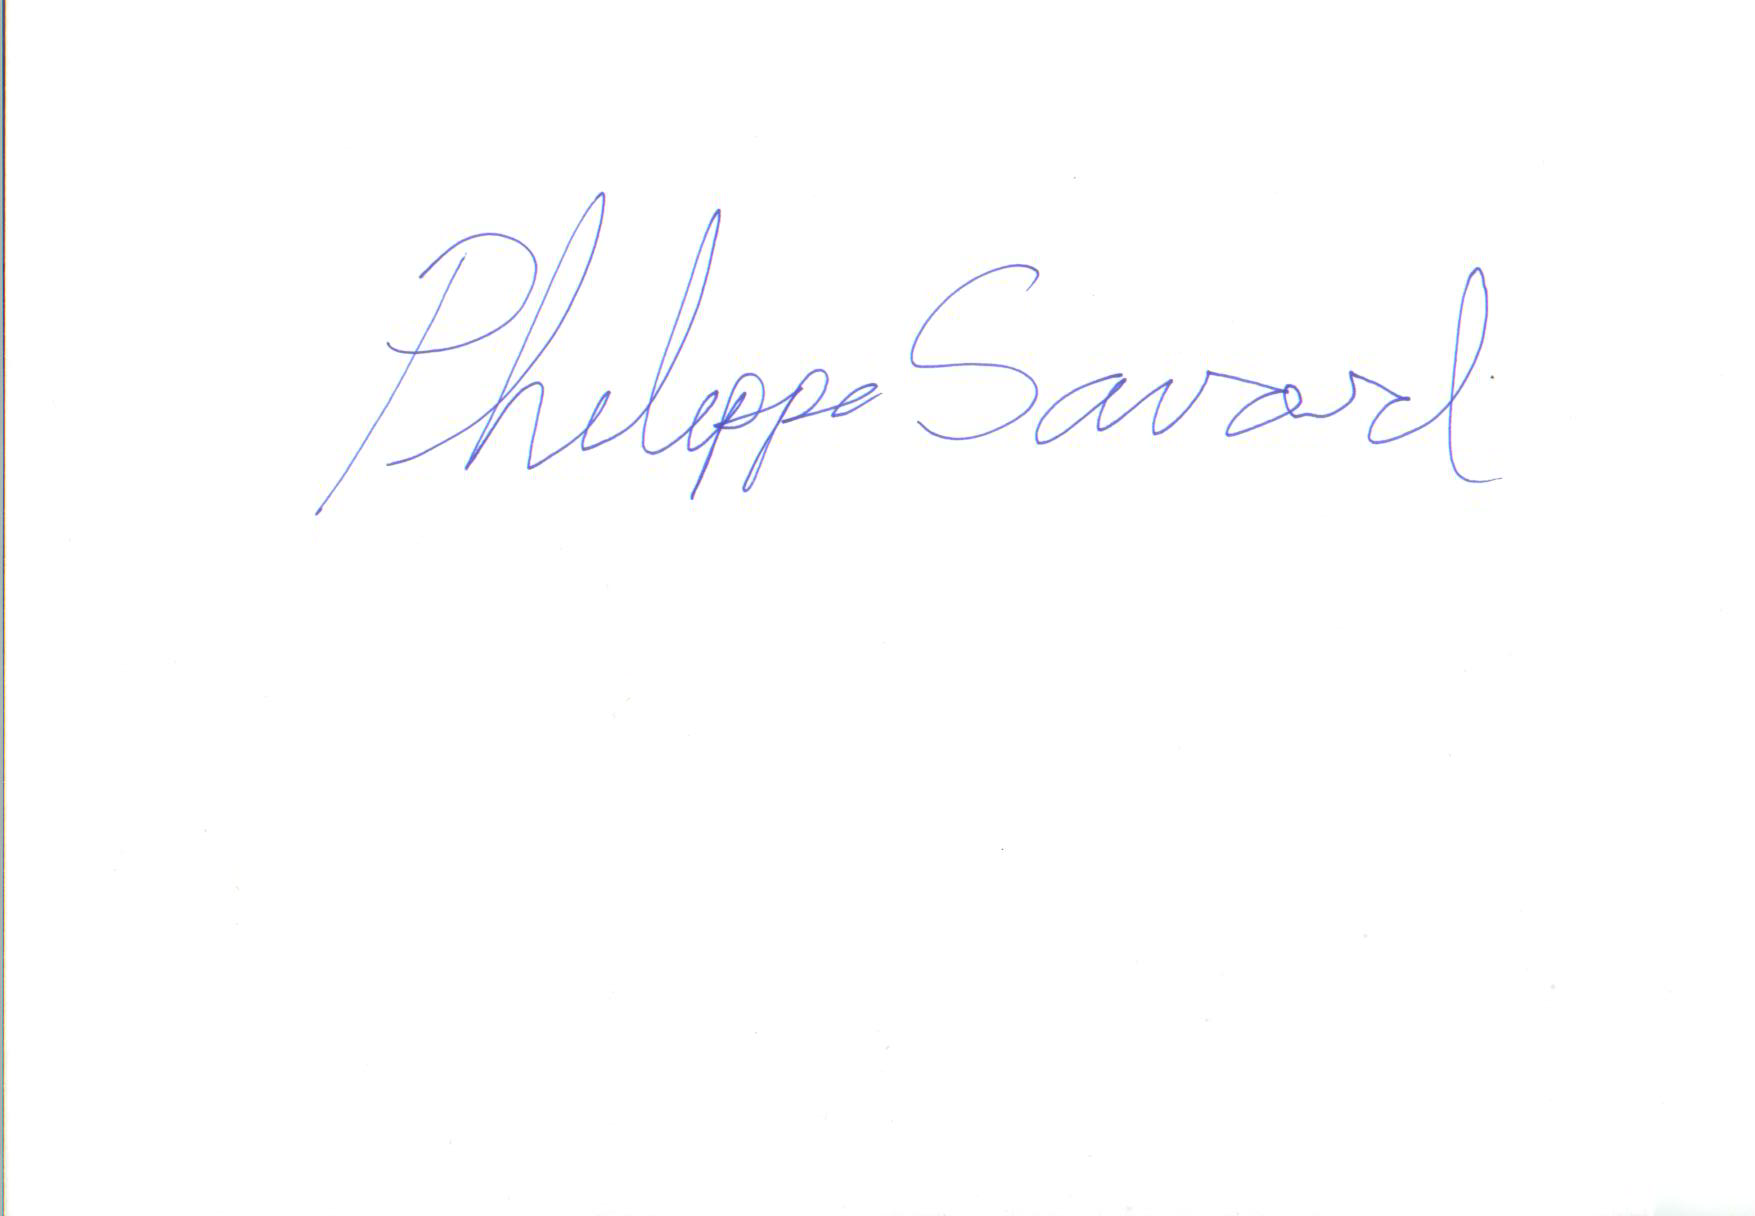
\includegraphics[width=4cm]{signature.png}
\end{center}

\end{document}